%% Based on a TeXnicCenter-Template by Gyorgy SZEIDL.
%%%%%%%%%%%%%%%%%%%%%%%%%%%%%%%%%%%%%%%%%%%%%%%%%%%%%%%%%%%%%

%------------------------------------------------------------
%
\documentclass{article}%
%Options -- Point size:  10pt (default), 11pt, 12pt
%        -- Paper size:  letterpaper (default), a4paper, a5paper, b5paper
%                        legalpaper, executivepaper
%        -- Orientation  (portrait is the default)
%                        landscape
%        -- Print size:  oneside (default), twoside
%        -- Quality      final(default), draft
%        -- Title page   notitlepage, titlepage(default)
%        -- Columns      onecolumn(default), twocolumn
%        -- Equation numbering (equation numbers on the right is the default)
%                        leqno
%        -- Displayed equations (centered is the default)
%                        fleqn (equations start at the same distance from the right side)
%        -- Open bibliography style (closed is the default)
%                        openbib
% For instance the command
%           \documentclass[a4paper,12pt,leqno]{article}
% ensures that the paper size is a4, the fonts are typeset at the size 12p
% and the equation numbers are on the left side
%
\usepackage{amsmath}%
\usepackage{amsfonts}%
\usepackage{amssymb}%
\usepackage{graphicx}
\usepackage{nameref}
\usepackage{url}
%-------------------------------------------
\newtheorem{theorem}{Theorem}
\newtheorem{acknowledgement}[theorem]{Acknowledgement}
\newtheorem{algorithm}[theorem]{Algorithm}
\newtheorem{axiom}[theorem]{Axiom}
\newtheorem{case}[theorem]{Case}
\newtheorem{claim}[theorem]{Claim}
\newtheorem{conclusion}[theorem]{Conclusion}
\newtheorem{condition}[theorem]{Condition}
\newtheorem{conjecture}[theorem]{Conjecture}
\newtheorem{corollary}[theorem]{Corollary}
\newtheorem{criterion}[theorem]{Criterion}
\newtheorem{definition}[theorem]{Definition}
\newtheorem{example}[theorem]{Example}
\newtheorem{exercise}[theorem]{Exercise}
\newtheorem{lemma}[theorem]{Lemma}
\newtheorem{notation}[theorem]{Notation}
\newtheorem{problem}[theorem]{Problem}
\newtheorem{proposition}[theorem]{Proposition}
\newtheorem{remark}[theorem]{Remark}
\newtheorem{solution}[theorem]{Solution}
\newtheorem{summary}[theorem]{Summary}
\newenvironment{proof}[1][Proof]{\textbf{#1.} }{\ \rule{0.5em}{0.5em}}

%----------------------------------------------------------
\newcommand{\vcenteredinclude}[1]{
\begingroup
\setbox0=\hbox{\includegraphics[width=0.06\textwidth]{#1}}
\parbox{\wd0}{\box0}\endgroup}
%----------------------------------------------------------

\begin{document}

\title{MatrixUser v2.2 User Guide}
\author{Fang Liu \\ (leoliuf@gmail.com)}
%\date{}
\maketitle

\tableofcontents

\section{What is MatrixUser}
Most of the medical images (e.g. CT, MRI, PET, etc.) comprises multiple frames which represent slices, phases, timing etc. from the same imaging object. Those images can be saved as multidimensional matrices in Matlab thanks to Matlab's powerful support of multidimensional data representation. However, within Matlab, most of image manipulation functions are limited or tailored for processing two-dimensional matrix. The MatrixUser is a software package which features functions designed and optimized specifically for manipulating multidimensional real or complex data matrix. MatrixUser provides a nice graphical environment for easily performing image analysis tasks including multidimensional image display, matrix (image stack) processing and rendering etc. MatrixUser is a great lightweight tool for users who are working in image processing field under Matlab.\\

The current MatrixUser version (v2.2) is made available at SourceForge website. MatrixUser is released as a free software. This means that you are free to use and modify this software as your needs, as long as you acknowledge the original author in any future work. If you find MatrixUser useful for the publication of any scientific results, including a line in your acknowledgments section referencing to MatrixUser and this belowing address is requested.\\
\\
MatrixUser downloading address:
\begin{center}
\url{https://sourceforge.net/projects/matrixuser/}
\end{center}

\section{Installing and Running MatrixUser}

To run MatrixUser, a Matlab installment is required. The current MatrixUser version has been tested under the following Matlab versions:
\begin{itemize}
\item Matlab R2011a 64-bit Windows
\item Matlab R2013a 64-bit Windows
\item Matlab R2012b 64-bit Unix
\end{itemize}

Installing and running MatrixUser is easy, you just need to download MatrixUser source code which is distributed as a compressed file, then extract the MatrixUser root folder, put the folder to any location in you computer. To run MatrixUser, start Matlab, then simply run the `Main.m' script under the MatrixUser root folder. \\

The MatrixUser main window (Figure \ref{fig:MatrixUser}) works as a matrix manager.

\begin{figure}[htbp]
	\centering
		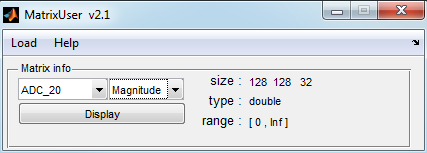
\includegraphics[width=0.8\textwidth]{Pictures/MatrixUser.eps}
	\caption{MatrixUser Main Window}
	\label{fig:MatrixUser}
\end{figure}


\section{Data Import}

Current MatrixUser version supports displaying any valid Matlab multi-dimensional matrix and Matlab structure variable. By default, MatrixUser reads Matlab base workspace, scans existing matrices in the Matlab session, then creates a matrix list for tracking matrix content. Once those matrices are updated by the user, MatrixUser will also update the matrix list. Moreover, there are several different approaches to import data from outside Matlab into MatrixUser. The imported matrices will be saved into Matlab base workspace. The import functions are located under `Load' menu, including:

	\begin{itemize}
	
	\item Load MAT file

The default Matlab .mat file is natively supported by MatrixUser.

	\item Load System Clipboard
	
If image content exists in the system clipboard, it can be converted into a RGB image which contains a three slice matrix with each slice corresponds to the individual Red, Green and Blue channel.

  \item Load ScreenShot

MatrixUser takes a full screenshot for current monitor and saves it into a RGB image as described above.
	
	\item Load from Binary file

Binary data file is supported by MatrixUser. The user needs to properly configure loading parameters (Figure \ref{fig:LoadFromBinary}) according to the matrix size and data type information.

\begin{figure}[htbp]
	\centering
		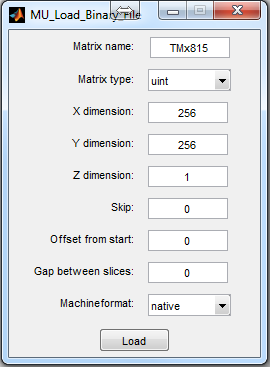
\includegraphics[width=0.4\textwidth]{Pictures/LoadFromBinary.eps}
	\caption{MatrixUser Binary File Loading Interface}
	\label{fig:LoadFromBinary}
\end{figure}	

 \item Load DICOM file(s)
		
MatrixUser supports loading multiple DICOM files by using a file filter interface (Figure \ref{fig:LoadFromDICOM}). The user needs to load DICOM files into the loading interface by selecting desired DICOM files (multiple selection supported). The selected files are listed in the DICOM file list. The user can click any single DICOM file to read associated DICOM header and image preview. To manually create a matrix using DICOM files, choose files from the DICOM file list, press `$>>>>>>$' to push the files into selected DICOM file list, provide a matrix name, press `Convert' button to create a matrix based on chosen DICOM files. The user can load those created matrices into base workspace by pressing `Load matrix' button.
		
\begin{figure}[htbp]
	\centering
		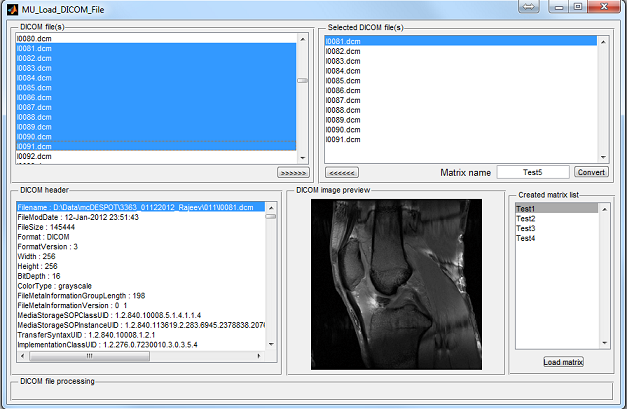
\includegraphics[width=0.8\textwidth]{Pictures/LoadFromDICOM.eps}
	\caption{MatrixUser DICOM File Loading Interface}
	\label{fig:LoadFromDICOM}
\end{figure}	

\item Load DICOM file(s) in Batch

MatrixUser supports loading DICOM files in a batch mode. This function requires the path of the folder containing DICOM files is provided. MatrixUser will try to create separate matrices for DICOM files coming from different image series. A matrix selection interface will provide converted matrices with loading functions.

\item Load from NIfTI file

NIfTI file with .nii suffix is supported by MatrixUser.
		
\end{itemize}


\section{Window Layout}

To activate MatrixUser display window, press `MatrixUser' button. If the selected matrix contains complex value, four options are available for displaying magnitude, phase, real and imaginary of the matrix. Figure \ref{fig:MatrixUserDisplayPanel} demonstrates an overview of the window layout of the MatrixUser display window. The window consists of 


\begin{figure}[htbp]
	\centering
		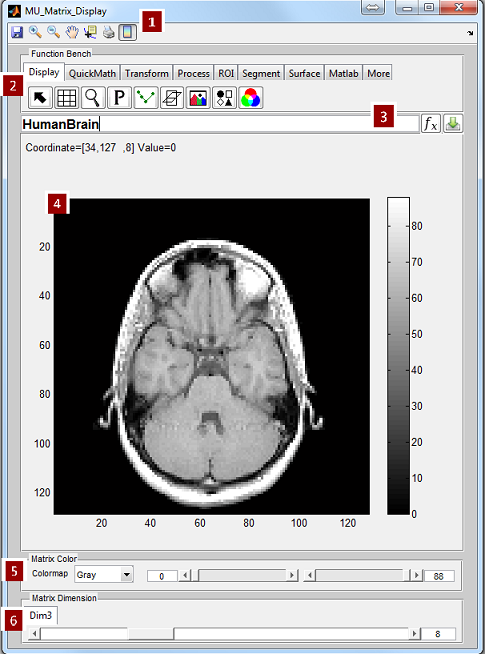
\includegraphics[width=0.8\textwidth]{Pictures/MatrixUserDisplayPanel.eps}
	\caption{MatrixUser Display Window}
	\label{fig:MatrixUserDisplayPanel}
\end{figure}


\begin{enumerate}

	\item Matlab Default Toolbar  \\
	
	Matlab toolbar provides basic interactive functions for displaying matrix. These functions include:
	
	\begin{itemize}
		\item \vcenteredinclude{Pictures/SaveFig.eps} : Save current image axes into an image file
		\item \vcenteredinclude{Pictures/ZoomIn.eps} : Zoom in matrix area
		\item \vcenteredinclude{Pictures/ZoomOut.eps} : Zoom out matrix area
		\item \vcenteredinclude{Pictures/Pan.eps} : Manually move matrix position
		\item \vcenteredinclude{Pictures/DataCursor.eps} : Check individual voxel value and index
		\item \vcenteredinclude{Pictures/Print.eps} : Print current figure
		\item \vcenteredinclude{Pictures/Colorbar.eps} : Turn on/off color bar
	\end{itemize}
	
	\item MatrixUser Function Library \\
	
	Most of the matrix analysis functions are represented on function bench panel. MatrixUser groups these functions into categories and dynamically loads them according to
	the dimension size and compatibility of current display matrix. A multi-tab is used to contain individual function button associated with each function. 
	The tabs under the multi-tab are used to switch between function categories, which include
	
	\begin{itemize}
		\item Display : Multi-dimensional matrix display functions
		\item QuickMath : Perform math calculation for current matrix
		\item Transform : Transform current matrix
		\item Process : Basic matrix processing functions
		\item ROI : Region-of-Interest functions
		\item Segment : Segmentation functions
		\item Surface : Generate surface or mesh plot for current image
		\item Matlab : Matlab default image tools
		\item More : Uncategorized functions
	\end{itemize}
	
	\item Matrix Calculator \\
	
The matrix calculator consists of three control items, including a matrix expression editbox, an execution button (\vcenteredinclude{Pictures/MatrixCalc.eps}) and a matrix saving button (\vcenteredinclude{Pictures/Upload.eps}). Valid matrix calculation expression can be executed in the calculator and updated in the display window, serving as a convenient way to analyze matrix calculation result. Matrix concatenation and recombination can also be done in the calculator, for example, to side-by-side compare multiple 3D matrices (Figure \ref{fig:MatrixCalcExample}). Some valid calculation examples are, but not limited to:
	\begin{itemize}
		\item A,B Combines A and B in one row
		\item A,B;C,D Combines A and B in the first row, C and D in the second row
		\item A,B;C,zeros(size(C)) Combines A and B in the first row, C in the second row, pad with zero value
		\item sin(A),cos(B) Calculates voxel-wise sin for A and cos for B, then combine them in one row
		\item A(:,1:10,:) Extracts submatrix from A and display it
	\end{itemize}
	
\begin{figure}[htbp]
	\centering
		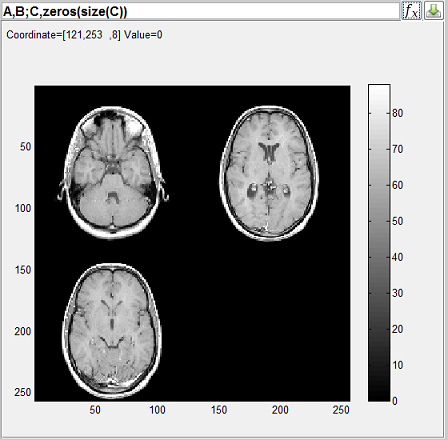
\includegraphics[width=0.6\textwidth]{Pictures/MatrixCalcExample.eps}
	\caption{MatrixUser Concatenation Example}
	\label{fig:MatrixCalcExample}
\end{figure}
	
where A, B, C and D are multi-dimensional matrices with proper matrix size. Also note that the source matrices have to stay in the base workspace for being referenced. Pressing the execution button will perform the calculation and save the result as a temporary matrix. The user can also save the temporary matrix into workspace by pressing matrix saving button. The saved temporary matrix will have a `\_tmp' suffix by default.
	
	\item Matrix Display Axes \\
	
The display axes renders an image for one slice of current matrix. The user can use mouse cursor to inspect the coordinate and value of any voxel. Moving mouse wheel back and forth moves the slice location along current dimension and updates the display axes.
	
	\item Matrix Color Control Group \\
	
	The matrix color control group provides a set of sliders, editboxes and popup menu which help control image color scheme and contrast. This group consists of
	
	\begin{itemize}
		\item Colormap Popup Menu: Choose different colormap scheme
		\item Upper Color Bound Slider (right slider): Slide to control the upper bound of color limits
		\item Upper Color Bound EditText (right editbox): Edit to control the upper bound of color limits
		\item Lower Color Bound Slider (left slider): Slide to control the lower bound of color limits
		\item Lower Color Bound EditText (left editbox): Edit to control the lower bound of color limits
	\end{itemize}
	
	\item Matrix Dimension Control Group \\
	
	MatrixUser measures the dimension size of the display matrix and assigns one slider and editbox for each dimension that is above 2 (i.e. no slider and editbox for the first and second dimension). These control items are located in individual dimension tab and can be used to switch among slices in current active dimension.
	
	\end{enumerate}
	
\section{Function Library}
	
	\begin{enumerate}

	\item Display \\
	
	Matrix display functions are listed under this tab. 
	
	\begin{itemize}
		\item \vcenteredinclude{Pictures/Release.eps} : Reset matrix display and erase additional display effect
		\item \vcenteredinclude{Pictures/Grid.eps} : Turn on and off black grid line on the image display axes
		\item \vcenteredinclude{Pictures/Axis.eps} : Configure axis mode
		\item \vcenteredinclude{Pictures/Magnifier.eps} : Open an instant magnifier which zooms in specific image area
		\item \vcenteredinclude{Pictures/LineProfile.eps} : Plot and update a profile curve along a resizable checking line (Figure \ref{fig:BrainProfile})
		
		\begin{figure}[htbp]
			\centering
				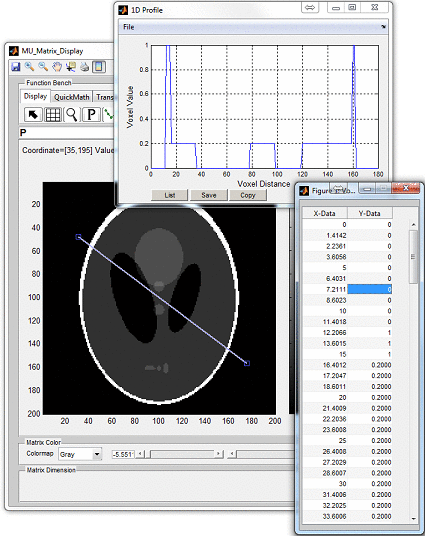
\includegraphics[width=0.7\textwidth]{Pictures/BrainProfile.eps}
			\caption{An Example of 1D Profile. The user can relocate and resize the profile checking line on the image for inspecting live 1D profile. The buttons on the profile window 
							 can list profile data, save the data as `data\_plt' array into workspace or copy the data into clipboard.}
			\label{fig:BrainProfile}
		\end{figure}	
		
		
		\item \vcenteredinclude{Pictures/DimProfile.eps} : Plot and update a profile curve along a matrix dimension (Figure \ref{fig:DimProfileWindow})
		
			\begin{figure}[htbp]
			\centering
				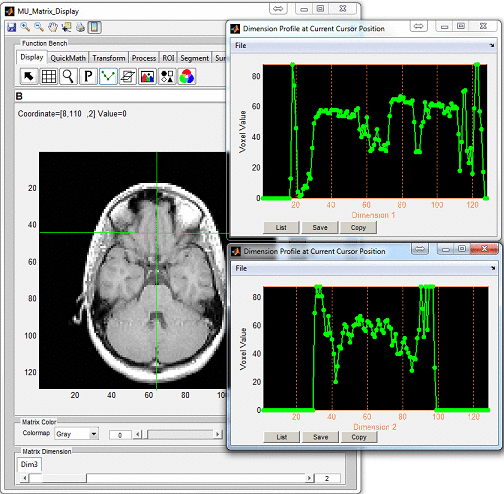
\includegraphics[width=0.8\textwidth]{Pictures/DimProfileWindow.eps}
			\caption{An Example of Plotting the First (Column) and Second (Row) Matrix Dimension Profile. The user needs to specify which matrix dimension to plot. The profile curve will update according to current mouse cursor position. The user can pause or resume live updating by right click on main display window.}
			\label{fig:DimProfileWindow}
		\end{figure}	
		
		\item \vcenteredinclude{Pictures/3DSlicer.eps} : Open a separate window with two matrix display axes (Figure \ref{fig:3DSlice}) displaying another two orthogonal images. The operation buttons on the second window consists of 

			\begin{itemize}
					\item \vcenteredinclude{Pictures/RedBar.eps} : Activate or deactivate localizer line on main display
					\item \vcenteredinclude{Pictures/YellowBar.eps} : Activate or deactivate localizer line on main display
					\item \vcenteredinclude{Pictures/Switch.eps} : Switch matrices between main display and second display. This operation simply permutes current matrix into its orthogonal version. The user can save the transformed matrix using (\vcenteredinclude{Pictures/Upload.eps}).
			\end{itemize}

			\begin{figure}[htbp]
				\centering
					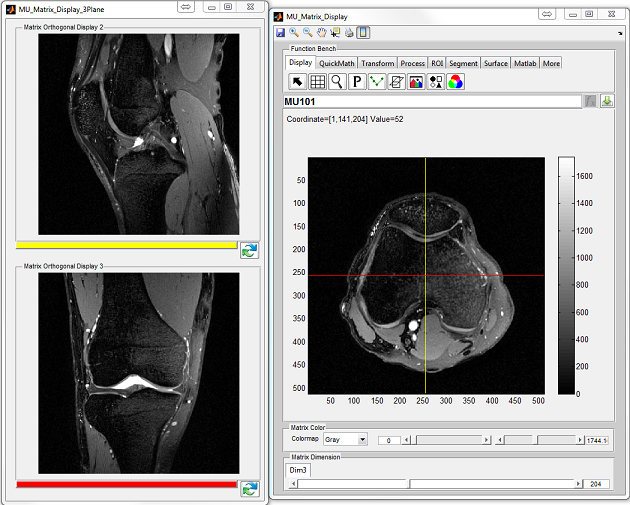
\includegraphics[width=0.8\textwidth]{Pictures/3DSlice.eps}
				\caption{3D Slicer. To change view slice, the user needs to activate localizer line and then click on desired coordinate on the main display window.}
				\label{fig:3DSlice}
			\end{figure}	

		\item \vcenteredinclude{Pictures/RGBImage.eps} : Create a RGB Image, assign current slice and following two slices to Red, Green and Blue channel, respectively
		\item \vcenteredinclude{Pictures/Montage.eps} : Create a montage image using multiple slices (Figure \ref{fig:MontageImage})
		
		\begin{figure}[htbp]
			\centering
				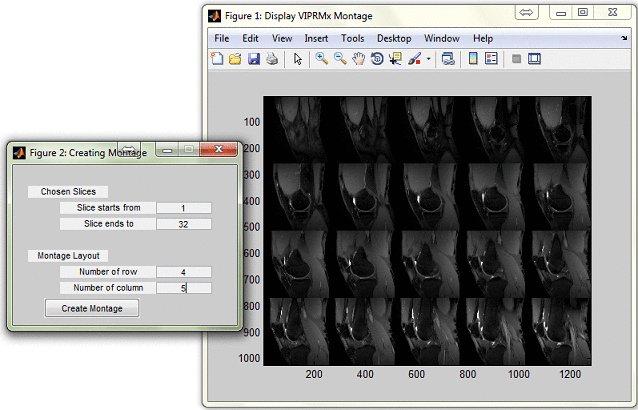
\includegraphics[width=0.8\textwidth]{Pictures/MontageImage.eps}
			\caption{Montage Image. An example of creating a 4-by-5 montage image using multiple matrix slices starting from the first slice.}
			\label{fig:MontageImage}
		\end{figure}
		
		\item \vcenteredinclude{Pictures/Fuse.eps} : Overlap two matrices with the same matrix size (Figure \ref{fig:ImageFuse}), notice that the user can press \vcenteredinclude{Pictures/Release.eps} to remove foreground matrix from overlapping with background matrix.
		
	\begin{figure}[htbp]
		\centering
			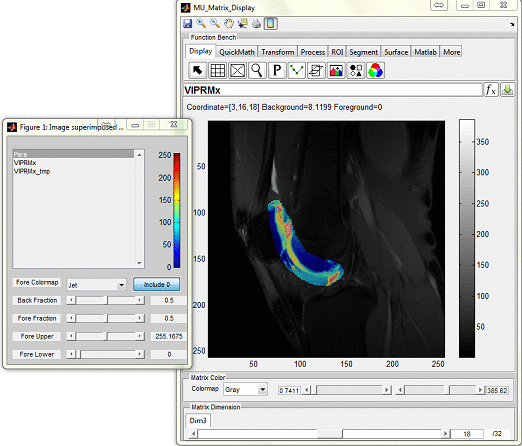
\includegraphics[width=1\textwidth]{Pictures/ImageFuse.eps}
		\caption{An Example of Overlapping Two Matrices. A second window is provided for adjusting overlapping effect. The user can choose to overlap any size compatible matrices from the matrix list. There exist control items to change foreground colormap scheme, to modify image intensity fraction, or to change foreground color limits.}
		\label{fig:ImageFuse}
	\end{figure}			
	
	\end{itemize}
	
	\item QuickMath \\
	
	This function category performs quick math calculation for current matrix. A few commonly used math calculation are provided under this tab. Instead, complex calculation can be performed using matrix calculator as mentioned above.
	
	\begin{itemize}
		\item \vcenteredinclude{Pictures/Abs.eps} : Calculate absolute value
		\item \vcenteredinclude{Pictures/Negnate.eps} : Calculate negative value
		\item \vcenteredinclude{Pictures/Ln.eps} : Calculate natural logarithm
		\item \vcenteredinclude{Pictures/Log.eps} : Calculate base 10 logarithm
		\item \vcenteredinclude{Pictures/Exp.eps} : Calculate exponential
		\item \vcenteredinclude{Pictures/10n.eps} : Calculate the power of 10
		\item \vcenteredinclude{Pictures/Sin.eps} : Calculate sine
		\item \vcenteredinclude{Pictures/Cos.eps} : Calculate cosine
		\item \vcenteredinclude{Pictures/Tan.eps} : Calculate tangent
		\item \vcenteredinclude{Pictures/ASin.eps} : Calculate inverse sine
		\item \vcenteredinclude{Pictures/ACos.eps} : Calculate inverse cosine
		\item \vcenteredinclude{Pictures/ATan.eps} : Calculate inverse tangent

	\end{itemize}
	
	\item Transform \\
	
		This function category performs spatial transformation or fast Fourier transform (FFT) to current matrix.
	
	\begin{itemize}
		\item \vcenteredinclude{Pictures/FlipLR.eps} : Flip matrix horizontally (along the first dimension)
		\item \vcenteredinclude{Pictures/FlipUD.eps} : Flip matrix vertically (along the second dimension)
		\item \vcenteredinclude{Pictures/FlipZ.eps} : Flip matrix along slice direction (the third dimension)
		\item \vcenteredinclude{Pictures/Rot90L.eps} : Rotate matrix 90 degree in the counter clockwise direction
		\item \vcenteredinclude{Pictures/Rot90R.eps} : Rotate matrix 90 degree in the clockwise direction
		\item \vcenteredinclude{Pictures/Rotate.eps} : Rotate matrix certain degree along an axis specified using the rotation axis origin and direction in the 3D space
		\item \vcenteredinclude{Pictures/Translate.eps} : Translate matrix along certain direction
		\item \vcenteredinclude{Pictures/FFT.eps} : Perform multi-dimensional FFT for current matrix, the user needs to specify up to which dimension to perform FFT.
	\end{itemize}
	
	
	\item Process \\
	
	This function category performs basic matrix processing functions.
	
	\begin{itemize}
		\item \vcenteredinclude{Pictures/Mask.eps} : Create binary mask according to given threshold
		\item \vcenteredinclude{Pictures/Smooth.eps} : Perform smoothing operation to current matrix
		\item \vcenteredinclude{Pictures/Sharpen.eps} : Perform sharpening operation to current matrix
		\item \vcenteredinclude{Pictures/Edge.eps} : Perform edge detection to current matrix
		\item \vcenteredinclude{Pictures/Filter.eps} : Provides various image filters (Figure \ref{fig:FilterResult})
		
		
	\begin{figure}[htbp]
		\centering
			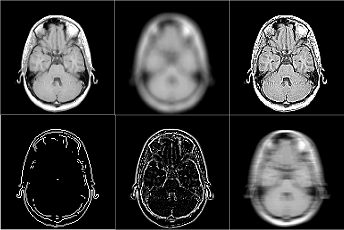
\includegraphics[width=0.6\textwidth]{Pictures/FilterResult.eps}
		\caption{Image Filters. An example is shown for applying various image filters.}
		\label{fig:FilterResult}
	\end{figure}
		
		
		\item \vcenteredinclude{Pictures/Noise.eps} : Add noise to matrix (Figure \ref{fig:NoiseResult})
		
	\begin{figure}[htbp]
		\centering
			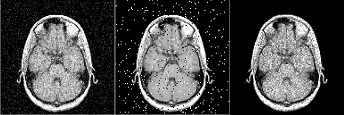
\includegraphics[width=0.6\textwidth]{Pictures/NoiseResult.eps}
		\caption{Image Noise. An example is shown for applying various image noise.}
		\label{fig:NoiseResult}
	\end{figure}
		
		
		\item \vcenteredinclude{Pictures/FillOut.eps} : Replace voxel value for the voxels within certain value range and outside a polygon area. The user needs to draw a polygon first (double click to confirm the polygon).
		\item \vcenteredinclude{Pictures/FillIn.eps} : Replace voxel value for the voxels within certain value range and inside a polygon area. The user needs to draw a polygon first (double click to confirm the polygon).
		\item \vcenteredinclude{Pictures/Fill.eps} : Replace voxel value for the voxels inside a polygon area. The user needs to draw a polygon first (double click to confirm the polygon).
		\item \vcenteredinclude{Pictures/Replace.eps} : Replace matrix area with a selected matrix source region. The user needs to draw a free-hand area (source region), drag the free-hand region to target matrix area, then double click to confirm the operation.
		\item \vcenteredinclude{Pictures/Crop.eps} : Crop current matrix using a rectangle box (double click to confirm the cropping)
		\item \vcenteredinclude{Pictures/Extract.eps} : Extract parts of current matrix using irregular shape (double click to confirm the extracting)
		\item \vcenteredinclude{Pictures/Resolution.eps} : Resample current matrix by using chosen interpolation method (Figure \ref{fig:ChangeResolution}). The user can specify sampling factors in x, y and z direction for 3D matrix.
		
	\begin{figure}[htbp]
		\centering
			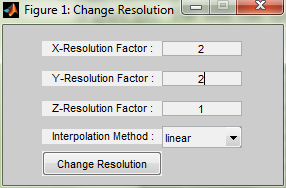
\includegraphics[width=0.5\textwidth]{Pictures/ChangeResolution.eps}
		\caption{Interpolation Window. An example is shown to double spatial resolution in x and y direction by using a linear interpolation.}
		\label{fig:ChangeResolution}
	\end{figure}
		
	\end{itemize}
	
	
	\item ROI \\
	
MatrixUser provides a set of function buttons for performing Region-of-Interest (ROI) analysis (Figure \ref{fig:ROIs}). To create a ROI, the user needs to click ROI button first, then draw a ROI on the image axes. The statistical measures (i.e. mean, standard deviation and relative standard deviation) for voxels in delineated ROI is calculated and updated with moving ROI position or changing ROI shape. The ROI function buttons consists of

	\begin{itemize}
		\item \vcenteredinclude{Pictures/FreeROI.eps} : Draw a free hand ROI
		\item \vcenteredinclude{Pictures/RectangleROI.eps} : Draw a rectangle or square ROI
		\item \vcenteredinclude{Pictures/CircleROI.eps} : Draw a circle or ellipse ROI
		\item \vcenteredinclude{Pictures/PolygonROI.eps} : Draw a polygon ROI
		\item \vcenteredinclude{Pictures/LineROI.eps} : Draw a straight line for measuring distance in units of pixels
		\item \vcenteredinclude{Pictures/AngleROI.eps} : Draw a polygon for measuring the interior angles in degrees
		\item \vcenteredinclude{Pictures/ROIManager.eps} : Record existing ROI shape and location into a ROI list, allow to redraw selected ROI in multiple image axes. To redraw a existing ROI, the user needs to select a ROI in the list, then press `Show' button. Note that the copied ROI is no longer resizable and movable.
		\item \vcenteredinclude{Pictures/Histogram.eps} : Plot histogram for current slice (Figure \ref{fig:Hist}); if ROIs exist, plot histogram for latest activated ROI. Histogram can be fitted by using multiple distribution types. For more complex fitting, Matlab built-in FitTool can be used.
	\end{itemize}
	
	\begin{figure}[htbp]
		\centering
			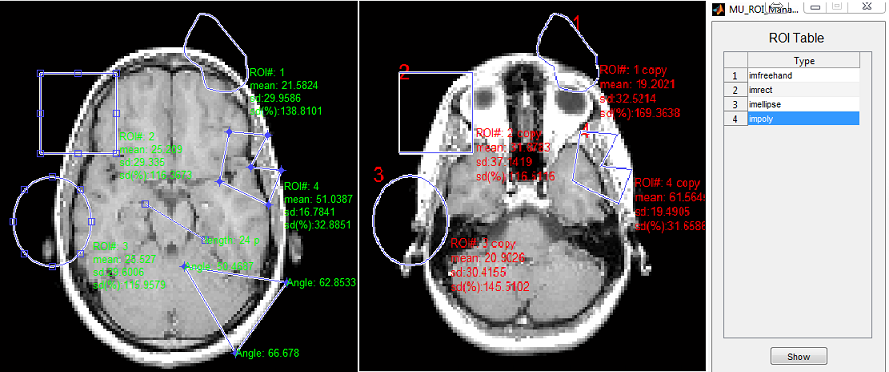
\includegraphics[width=1\textwidth]{Pictures/ROIs.eps}
		\caption{Draw Multiple ROIs and Redraw on A Second Image. The source ROIs are in green, copied ROIs are in red.}
		\label{fig:ROIs}
	\end{figure}
	
	
	\begin{figure}[htbp]
		\centering
			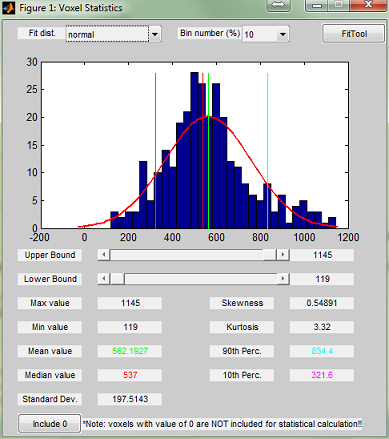
\includegraphics[width=0.6\textwidth]{Pictures/Hist.eps}
		\caption{Histogram for One Image Slice}
		\label{fig:Hist}
	\end{figure}
	
	\item Segment \\
	
MatrixUser supports functions for performing multi-slice manual segmentation. To create a segmentation, click segmentation button, then draw a region on the image axes. The user can modify the region location and shape prior to confirming segmentation with double click. The segmentation buttons consists of
	
	\begin{itemize}
		\item \vcenteredinclude{Pictures/FreeSeg.eps} : Do a free-hand segmentation
		\item \vcenteredinclude{Pictures/CircleSeg.eps} : Do a circle or ellipse segmentation
		\item \vcenteredinclude{Pictures/PolygonSeg.eps} : Do a polygon segmentation
		\item \vcenteredinclude{Pictures/EditSeg.eps} : Edit segmentation
		\item \vcenteredinclude{Pictures/SaveSeg.eps} : Save segmentation into a MAT file
		\item \vcenteredinclude{Pictures/LoadSeg.eps} : Load segmentation from a MAT file
	\end{itemize}
	
	
\begin{figure}[htbp]
	\centering
		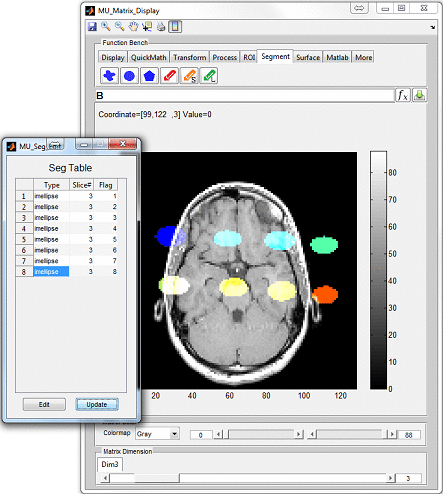
\includegraphics[width=0.8\textwidth]{Pictures/Segs.eps}
	\caption{Editing Segmentation}
	\label{fig:Segs}
\end{figure}	

To edit segmented region (Figure \ref{fig:Segs}), press \vcenteredinclude{Pictures/EditSeg.eps} to open a segmentation manager. The manager records the type and location for existing segmented regions. The user can click any region item to inspect the location of the region. To edit chosen region, click `Edit' button to activate the region outline. Both the shape and mask flag are editable for segmented region. After editing, click `Update' to conform modification. The user can press \vcenteredinclude{Pictures/SaveSeg.eps} to save current segmentation into a MAT file which contains a mask matrix and a cell array storing segmentation location information. The user can also press \vcenteredinclude{Pictures/Upload.eps} to save the mask matrix into workspace. Pressing \vcenteredinclude{Pictures/LoadSeg.eps} can load previous segmented regions from a saved MAT file. Notice that the user can press \vcenteredinclude{Pictures/Release.eps} to remove segmentation from overlapping with background matrix. 
	
	\item Surface \\
	
	This function category generates surface or mesh plot for current image.
	
		\begin{itemize}
		\item \vcenteredinclude{Pictures/Contour.eps} : Create contour plot of current matrix
		\item \vcenteredinclude{Pictures/Contour3.eps} : Create 3D contour plot of current matrix
		\item \vcenteredinclude{Pictures/ContourFill.eps} : Create filled 2D contour plot
		\item \vcenteredinclude{Pictures/Surface.eps} : Create 3D shaded surface plot
		\item \vcenteredinclude{Pictures/SurfaceCon.eps} : Create surface plot and contour
		\item \vcenteredinclude{Pictures/SurfaceCol.eps} : Create surface plot with colormap based lighting
		\item \vcenteredinclude{Pictures/Mesh.eps} : Create mesh plot
		\item \vcenteredinclude{Pictures/MeshCon.eps} : Create mesh plot and contour
		\item \vcenteredinclude{Pictures/MeshC.eps} : Create a curtain around a mesh plot
		\item \vcenteredinclude{Pictures/Reb.eps} : Create a ribbon plot
		\item \vcenteredinclude{Pictures/Waterfall.eps} : Create a waterfall plot
		\item \vcenteredinclude{Pictures/Pcolor.eps} : Create pcolor (checkerboard) plot
	\end{itemize}
	
	
	\item Matlab \\
	
	Matlab default image tools (Figure \ref{fig:matlabIM}) are tailored for MatrixUser and included in this category.
	
		\begin{itemize}
		\item \vcenteredinclude{Pictures/imtool.eps} : Perform imtool for current image
		\item \vcenteredinclude{Pictures/immovie.eps} : Perform immovie for playback current 3D matrix
		\item \vcenteredinclude{Pictures/imcontrast.eps} : Perform imcontrast for adjusting image contrast
    \end{itemize}
		
\begin{figure}[htbp]
	\centering
		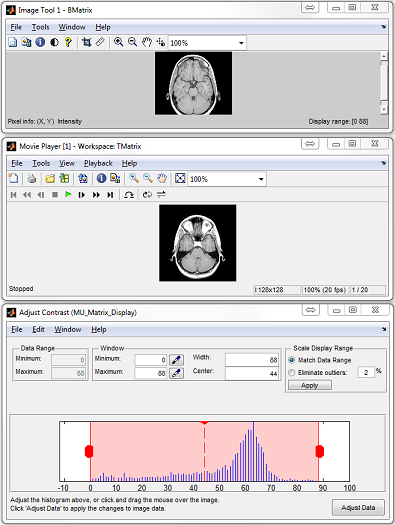
\includegraphics[width=0.7\textwidth]{Pictures/matlabIM.eps}
	\caption{Matlab Tools}
	\label{fig:matlabIM}
\end{figure}	
	
	\item More \\

	Uncategorized functions are categorized under this tab.
	
	\begin{itemize}
		\item \vcenteredinclude{Pictures/3DRender.eps} : Create a 3D graph for rendering current matrix (Figure \ref{fig:BrainRender})
		
		\begin{figure}[htbp]
			\centering
			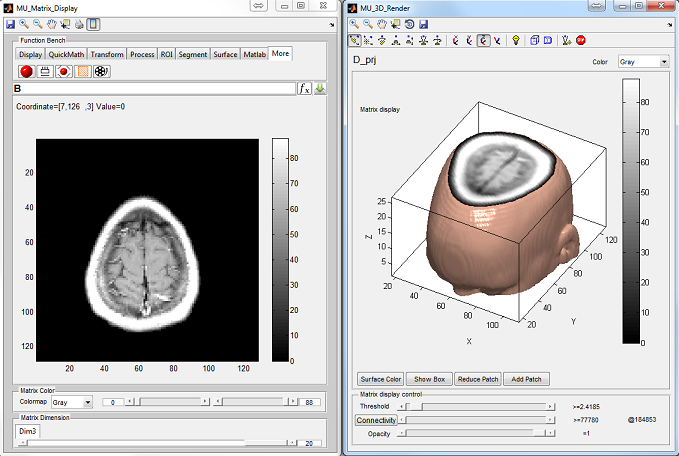
\includegraphics[width=1\textwidth]{Pictures/BrainRender.eps}
			\caption{An Example of 3D Human Brain Rendering. Control units on the rendering window are provided for fine tuning the renderer. The user can select isosurface threshold, cutoff connectivity threshold (i.e. object with total voxels less than the threshold will be removed from the rendering. `@' is followed by the voxel number of current largest object) and object opacity. A set of pushbuttons are also available for changing surface color, display box and patches. The default Matlab camera toolbar are provided for adjusting the lighting effect.}
			\label{fig:BrainRender}
		\end{figure}	
		
		\item \vcenteredinclude{Pictures/MIP.eps} : Perform projection along a given matrix dimension. Support multi-dimensional matrix projection
		\item \vcenteredinclude{Pictures/MIP3D.eps} : Perform 3D projection along x, y or z axis with certain angle increment (Figure \ref{fig:3DMIP})
		
		
		\begin{figure}[htbp]
			\centering
				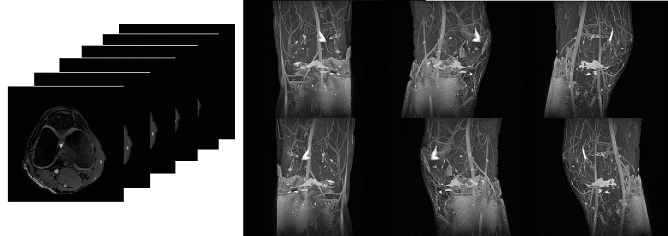
\includegraphics[width=1\textwidth]{Pictures/3DMIP.eps}
			\caption{3D Maximum Intensity Projection (MIP). An example of 3D MIP around axial axis of a human knee MRI image stack shows the vascular system of the knee joint.}
			\label{fig:3DMIP}
		\end{figure}	
		
		\item \vcenteredinclude{Pictures/3DReslice.eps} : Reslice 3D matrix at given direction. The user needs to draw a line for indicating the slicing direction with double click for confirmation (Figure \ref{fig:Reslice})
		\item \vcenteredinclude{Pictures/Moive.eps} : Create a movie using current matrix display. Support making movie for overlapped matrices.
	\end{itemize}
	
		\begin{figure}[htbp]
		\centering
			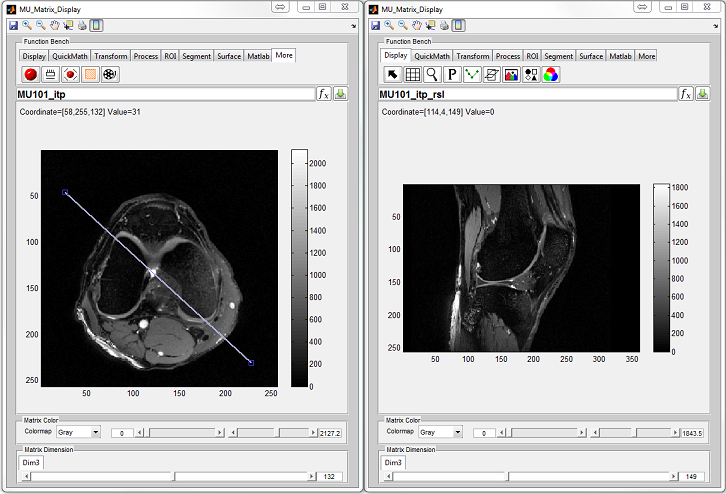
\includegraphics[width=1\textwidth]{Pictures/Reslice.eps}
		\caption{Reslice 3D Matrix. An example of 3D reslicing generates a new stack of images in the oblique plane from an axial human knee MRI image stack. Note that the resliced images are extracted from the plane perpendicular to the indicating line on the left window.}
		\label{fig:Reslice}
	\end{figure}	
	
\end{enumerate}
	
\end{document}
